\documentclass[./main.tex]{subfiles}

\begin{document}
\section{Models}
The following section covers the theory behind the various models that will be introduced in Section \ref{sec:experiments}.

\subsection{Mask R-CNN}
\begin{figure}[htbp]
    \centering
    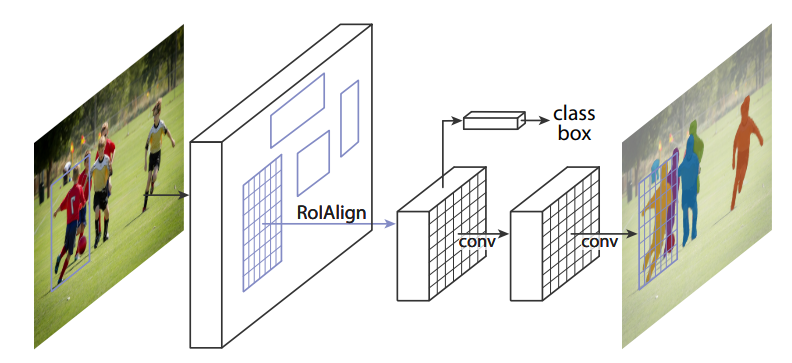
\includegraphics[height=5cm]{./entities/mask_rcnn.PNG}
    \caption{The Mask R-CNN framework for instance segmentation \cite{https://doi.org/10.48550/arxiv.1703.06870}.}
    \label{fig:mask_rcnn}
\end{figure}
\noindent When we will be performing the pose estimation in Section \ref{sec:experiments}, our developed methods will be a variation of the \textit{Mask R-CNN}, introduced by He \textit{et al.} in 2018 \cite{https://doi.org/10.48550/arxiv.1703.06870}. The following subsection explains the architecture of the Mask R-CNN and is based on an interpretation of He \textit{et al.} \cite{https://doi.org/10.48550/arxiv.1703.06870} and Zhang \cite{mask_rcnn_explained}.

\subsection{UniPose-LSTM}

\subsection{DeciWatch}

\end{document}